\section{Application to mechanical systems}
We will now proceed by using a mechanical `prototype' example for our mechanical system: the harmonic oscillator with \emph{two} dampers: one in series and one in parallel. The two dampers are interesting because they completely fill the state transition matrix: as such, this system can represent all the possible cases discussed in the previous section. Furthermore, the two dampers have a very distinctive interpretation within the field of economic engineering.
%\begin{figure}[ht!]
%    \centering
%    \begin{tikzpicture}[every node/.style={outer sep=0pt,thick}]
    % Spring style
    \tikzstyle{spring} = [thick, 
                          decorate,
                          decoration={zigzag,pre length=0.2cm,post length=0.2cm,segment length=6}]

    % Damper style
    \tikzstyle{damper}= [thick, 
                         decoration={markings,  
                         mark connection node=dmp,
                         mark=at position 0.5 with 
                         {
                           \node (dmp) [thick,inner sep=0pt,transform shape,rotate=-90,minimum width=15pt,minimum height=3pt,draw=none] {};
                           \draw [thick] ($(dmp.north east)+(2pt,0)$) -- (dmp.south east) -- (dmp.south west) -- ($(dmp.north west)+(2pt,0)$);
                           \draw [thick] ($(dmp.north)+(0,-5pt)$) -- ($(dmp.north)+(0,5pt)$);
                         }
                        }, decorate]
                        
    \tikzstyle{ground} = [fill, 
                          pattern = north east lines, 
                          draw = none,
                          minimum width = 0.75cm,
                          minimum height = 0.3cm]

    \node (M) [draw,minimum width=1cm, minimum height=1.5cm] {$m$};

    \node (ground) [ground,anchor=north,yshift=-0.25cm,minimum width=1.5cm] at (M.south) {};
    \draw (ground.north east) -- (ground.north west);
    \draw [thick] (M.south west) ++ (0.2cm,-0.125cm) circle (0.125cm)  (M.south east) ++ (-0.2cm,-0.125cm) circle (0.125cm);

    \node (wall) [ground, rotate=-90, minimum width=2.5cm,yshift=-3cm] {};
    \node [xshift=-1.2cm, circle, fill=black, inner sep = 1pt] (p1) at ($(M.north west)!(wall.160)!(M.south west)$) {};
    %\node [yshift=0.3cm] at (p1) {$q_1$};
    \draw (wall.north east) -- (wall.north west);
    %\node[anchor=south] at (M.north) {$q_2$};

    \node[above=1.5cm of wall, outer sep = 0mm, inner sep=0mm] (p3) {};
    \node[above=2.3cm of wall, outer sep = 0mm, inner sep=0mm] (p4) {};


    \path (p3) -| node[outer sep = 0mm, inner sep=0mm] (p5) {} (p1);
    \path (p4) -| node[outer sep = 0mm, inner sep=0mm] (p6) {} (M);

    \draw[|->] (p3) -- (p5) node[anchor=south,pos=0.5] {$q$};
    \draw[|->] (p4) -- (p6) node[anchor=south,pos=0.5] {$q_1$};

    \draw (p5) ++(0, 0.2) -- ++(0,-1.2);
    \draw (p6) ++(0, 0.2) -- ++(0,-1.7);

    %\node (coord1) [yshift=1.5cm, minimum width=0.3cm] at (wall) {};
    %\draw[->] (coord1) -- ++(1cm, 0);

    \draw [spring] (wall.160) -- (p1) node[pos=0.5,anchor=south, outer sep=4pt] {$k$};
    \draw [damper] (wall.20) -- ($(M.north west)!(wall.20)!(M.south west)$) node[pos=0.5, anchor=north, outer sep=8pt] {$b_p$};
    \draw[damper] (p1) -- ($(M.north west)!(wall.160)!(M.south west)$) node[pos=0.5, anchor=south, outer sep=8pt] {$b_s$};


    \node[bgelement, label=west:$q$] (J0) at (3.5, 0.5) {0};

    \node[bgelement, label=east:$p$] (J1) at (5, 0.5) {1};

    \node[bgelement, label=north:$k$] (C) at (3.5, 2) {C};
    \node[bgelement, label=south:$b_s$] (Rs) at (3.5, -1) {R};

    \node[bgelement, label=north:$m$]  (I) at (5, 2) {I};
    \node[bgelement, label=south:$b_p$]  (Rp) at (5, -1) {R};

    % test
    \draw[bonds] 
        (J1) edge[e_out] (I)
        (J1) edge[f_out] (Rp)

        (J0) edge[f_out] (C)
        (J0) edge[e_out] (Rs)
        (J0) edge[e_out] (J1);

\end{tikzpicture}

%    \caption{Schematic of the harmonic oscillator with two dampers: one in series and one in parallel.}
%    \label{fig:double_damped_osc}
%\end{figure}

\subsection{Equations of motion}
The harmonic oscillator with two dampers is shown in \cref{fig:double_damped_osc}. The equations of motion can be readily derived:
\begin{equation}
    \begin{split}
        m\ddot{q}_1 &= -kq - b_p \dot{q}_1 \\
        kq &= b_s(\dot{q}_1 - \dot{q}) \\
    \end{split}
\end{equation}
Due to the presence of the serial damper, the situation is somewhat curious, since there are two positions in the system; one measuring the spring deflection $q$ and the position of the mass $q_1$. However, the node connecting the serial damper and the spring has no mass, and therefore no second-order dynamics: as such, the overall order of the system is 2. In accordance with the economic analogy, we will say that position is stored in the spring, but momentum is stored in a mass. Hence, let $p = m\dot{q}_1$ --- but $\dot{q} \neq p/m$ in general. The equations of motion then have the matrix form:
\begin{equation*}
    \mqty(\dot{q}\\\dot{p}) = \mqty(-\tfrac{k}{b_s} & \tfrac{1}{m} \\ -k & - \tfrac{b_p}{m})\mqty(q \\ p),
\end{equation*}
or, using the parameters defined in \cref{tab:ddho_params}:
\begin{equation}
    \mqty(\dot{q}\\\dot{p}) = \underbrace{\mqty(-\gamma_s & \frac{1}{m} \\ -m\Omega_n^2 & - \gamma_p)}_A \mqty(q \\ p).
    \label{eq:ddho_eom}
\end{equation}
The nontrivial relation between momentum and the $\dot{q}$ also precludes us from casting this system directly to the Lagrangian formalism, because the vector field is not second-order. A second-order vector field implies that the `velocities' really are the time derivatives of the `positions', (cf. \cref{app:symplectic_geometry} for a more formal discussion).

%\begin{table}[ht!]
%    \caption{Substition parameters for the harmonic oscillator with serial and parallel damping, shown in \cref{fig:double_damped_osc}.}
%    \label{tab:ddho_params}
%    \centering
%    \begin{tabular}{llll}
%        \toprule
%        \textbf{Name} & \textbf{Symbol} & \textbf{Value} & \textbf{Units} \\
%        \midrule
%            Serial damping coefficient & $\gamma_s$ & $k/b_s$ & \si{\per \second} \\
%            Parallel damping coefficient & $\gamma_p$ & $b_p/m$ & \si{\per \second} \\
%            Natural frequency & $\Omega_n$ & $\sqrt{k/m}$ & \si{\per \second} \\
%            Damped frequency & $\Omega_d$ &  & \si{\per \second} \\
%        \bottomrule
%    \end{tabular}
%\end{table}

The split-quaternion associated with the $A$-matrix of the doubly damped system can easily be found using the mapping defined by \cref{eq:inv_quat_isom}. We must, however, be careful when dealing with physical systems, because the entries of the $A$-matrix are not dimensionless. In a vector space, we associate the units with the basis vectors, not with the components. For example, in a two-dimensional vector space spanned by a axis for apples and and an axis for pears, and we wish to represent that someone possesses three apples and four pairs, the \emph{components} of that vector are $(3, 4)$, and the \emph{unit vectors} are $(1 \text{ apple}, 1\text{ pear})$. Along the same line, we must define the units in the $A$-matrix in the split-quaternion basis elements 1, \quati, \quatj, \quatk. To do so, we define the reference quantities and $m_0, t_0$. The basis elements are then mapped in terms of these reference quantities:
$$ 
    \phi(1) = \mqty(\tfrac{1}{t_0} & 0 \\ 0 & \tfrac{1}{t_0}), \quad 
    \phi(\quati) = \mqty(0 & \tfrac{1}{m_0} \\  -\tfrac{m_0}{t_0^2} & 0), \quad
    \phi(\quati) = \mqty(0 & \tfrac{1}{m_0} \\  \tfrac{m_0}{t_0^2} & 0), \quad
    \phi(\quatk) = \mqty(\tfrac{1}{t_0} & 0 \\ 0 & -\tfrac{1}{t_0}), \quad 
$$
where, in case we would use SI units, $m_0 = \SI{1}{\kilogram}$ and $t_0 = \SI{1}{\second}$. As a result, the split-quaternion associated with the $A$-matrix given in \cref{eq:ddho_eom} becomes
\begin{equation}
    a\:=\: -\frac{1}{2}\qty(t_0\gamma_s + t_0\gamma_p)\:+\:\frac{1}{2}\qty(\frac{m_0}{m} + \frac{m\Omega_n^2 t_0^2}{m_0})\quati\:+\:\frac{1}{2}\qty(\frac{m_0}{m} + \frac{m\Omega_n^2 t_0^2}{m_0})\quatj\:+\:\frac{1}{2}\qty(t_0\gamma_p - t_0\gamma_s)\quatk. 
    \label{eq:ddho_quat_units}
\end{equation}
Clearly, all the components of the split-quaternion are dimensionless. This really is not too wild of an idea: after all, we are translating the matrix itself, and \emph{not} the two-dimensional vector space that it acts on. The units are inherited from the vector space, so we should only add them when returning from the split-quaterions back to the realm of the matrices. 

The preceding argument only explains why we can work around this issue without performing illegal operations, but it does not give a satisfactory answer as to why we would be interested to add numbers that are seemingly incompatible. Indeed, observe that $\gamma_s$ and $\gamma_p$ have the same units, whereas $\tfrac{1}{m}$ and $\Omega_n^2$ do not. So, in which sense can the $\quati$ and $\quatj$-components be of any signficance? To answer this question, we first note that `rescaling of units' is a linear operation on the vector space given by a diagonal matrix (with nonzero diagonal entries): 
$$ N = \mqty(\dmat[0]{\nu_1}{\nu_2}) \qquad \nu_1, \nu_2 \in \real^*, $$
which form the group isomorphic to $(\real^*)^2$. This transformation of the vector space manifests itself on the $A$-matrix as: $ A' = N^{-1}A N$. It is easy to see that the basis matrices (or vector fields) for `1' and \quatk are invariant under this transformation, while the \quati and \quatj-matrices are not (that is, without making use of the reference quantities). A geometric explanation is that the eigenvectors of the identity matrix and the \quatk-matrix point along the axes; and are therefore invariant under rescaling of these axes. As a result of this fact, the \quati and \quatj components will not transform properly under a unit transformation. It is common practice in physics to rescale the state space of the undamped harmonic oscillator as follows \cite{Dekker1981,Dedene1980}
$$ p \mapsto \frac{p}{m} \qquad q \mapsto m\Omega q, $$
such that the Hamiltonian reverts to a particularly convenient form. We can see that this is precisely the transformation that kills the \quatj-component of the split-quaternion. This would essentially resolve this `unit problem', because it only arises when we attempt to make the \emph{distinction} between the \quati and \quatj-component.

In contrast to common practice in physics, we are interested in the full range of geometrical properties that the trajectories in the phase plane can exhibit, including those that are not invariant under the action of the structure group $(\real^*)^2$ that contains the changes of units. Furthermore, many invariants, such as the split-quaternion (vector) norm, scalar part, etc. that we use to draw conclusions about the nature of the system \emph{do} commute with this group action, and are therefore remain valid. It is even possible to effect unit transformations within the split-quaternion transformations by translating the matrix $N$ to the appropriate split-quaternion using the isomorphism. We can indeed observe that the action of $n^{-1} a n$ (where $n = \phi^{-1}(n)$) produces a split-quaternion with zero $\quatj$-component. 

As a final argument, we can say that the `rescaling of the axes', while common in physics and mathematically allowed, is of little use for engineers, since they tend to stick to SI units in the first place. The `scale of the axes' is therefore a physical reality. This is why we choose not to discard the $\quatj$-component through a rescaling.

To conclude, it is not so much the case that unit transformations are not allowed in the split-quaternion space, but the question as to what the units of the \quatj-components are is moot. Unfortunately, the notation in \cref{eq:ddho_quat_units} is rather obfuscating. Hence, we take the freedom to choose $m_0 = 1 (\si{\kilogram})$ and $t_0 = 1 (\si{\second})$, and write the split-quaternion as follows:
\begin{equation}
    a\:=\: -\tfrac{1}{2}\qty(\gamma_s + \gamma_p)\:+\:\tfrac{1}{2}\qty(\tfrac{1}{m} + m\Omega_n^2)\quati\:+\:\tfrac{1}{2}\qty(\tfrac{1}{m} + m\Omega_n^2)\quatj\:+\:\tfrac{1}{2}\qty(\gamma_p - \gamma_s)\quatk. 
    \label{eq:ddho_quat}
\end{equation}
This of course requires the implicit understanding that all the components are dimensionless, and that we are not just adding apples and pears. 

\subsection{Eigenvalues}
Underdamped, overdamped critically damped.

\subsection{Eigenvector geometry in SO(3, R)}
We have learned in \cref{ssec:quat_isomorphism} that the eigenvalues of a $2\times 2$-matrix can be expressed in terms of the scalar part and vector norm of the associated split-quaternion. Once we have removed the scalar part and normalized the vector part with its norm (if admissible), we are left with the unit vector part of the split-quaternion. Hence, this two-dimensional object contains the remaining information present in the matrix: the eigenvectors. The great advantage of split-quaternions is that the unit vector is entirely unambiguous, which is not the case for eigenvectors, for they represent only a direction, while the length of the eigenvector is arbitrary. The unit vector part of the split-quaternion encodes this information in a \emph{single two-dimensional object}.

As mentioned in \cref{ssec:quat_basics}, the split-quaternion vectors live in the Lorentzian three-space $\real^{1, 2}$. The \emph{unit vectors} in this space live in a particular subspace, the Lorentzian equivalent of the unit sphere in this space. Due to the indefiniteness of the Lorentz norm, this subspace is disconnected: it consists out of three connected parts (shown in \cref{fig:hyperboloids}):
\begin{itemize}
    \item The \emph{one-sheet hyperboloid}, which contains all the \emph{spacelike} unit vectors (overdamped systems).
    \item The \emph{light cone}, which contains all the \emph{lightlike} vectors (the notion of a unit vector is not well defined in this region) (critically damped systems).
    \item The \emph{two-sheet hyperboloid}; which contains all the \emph{timelike} unit vectors (underdamped systems).
\end{itemize}

\begin{figure}[ht!]
    \centering
    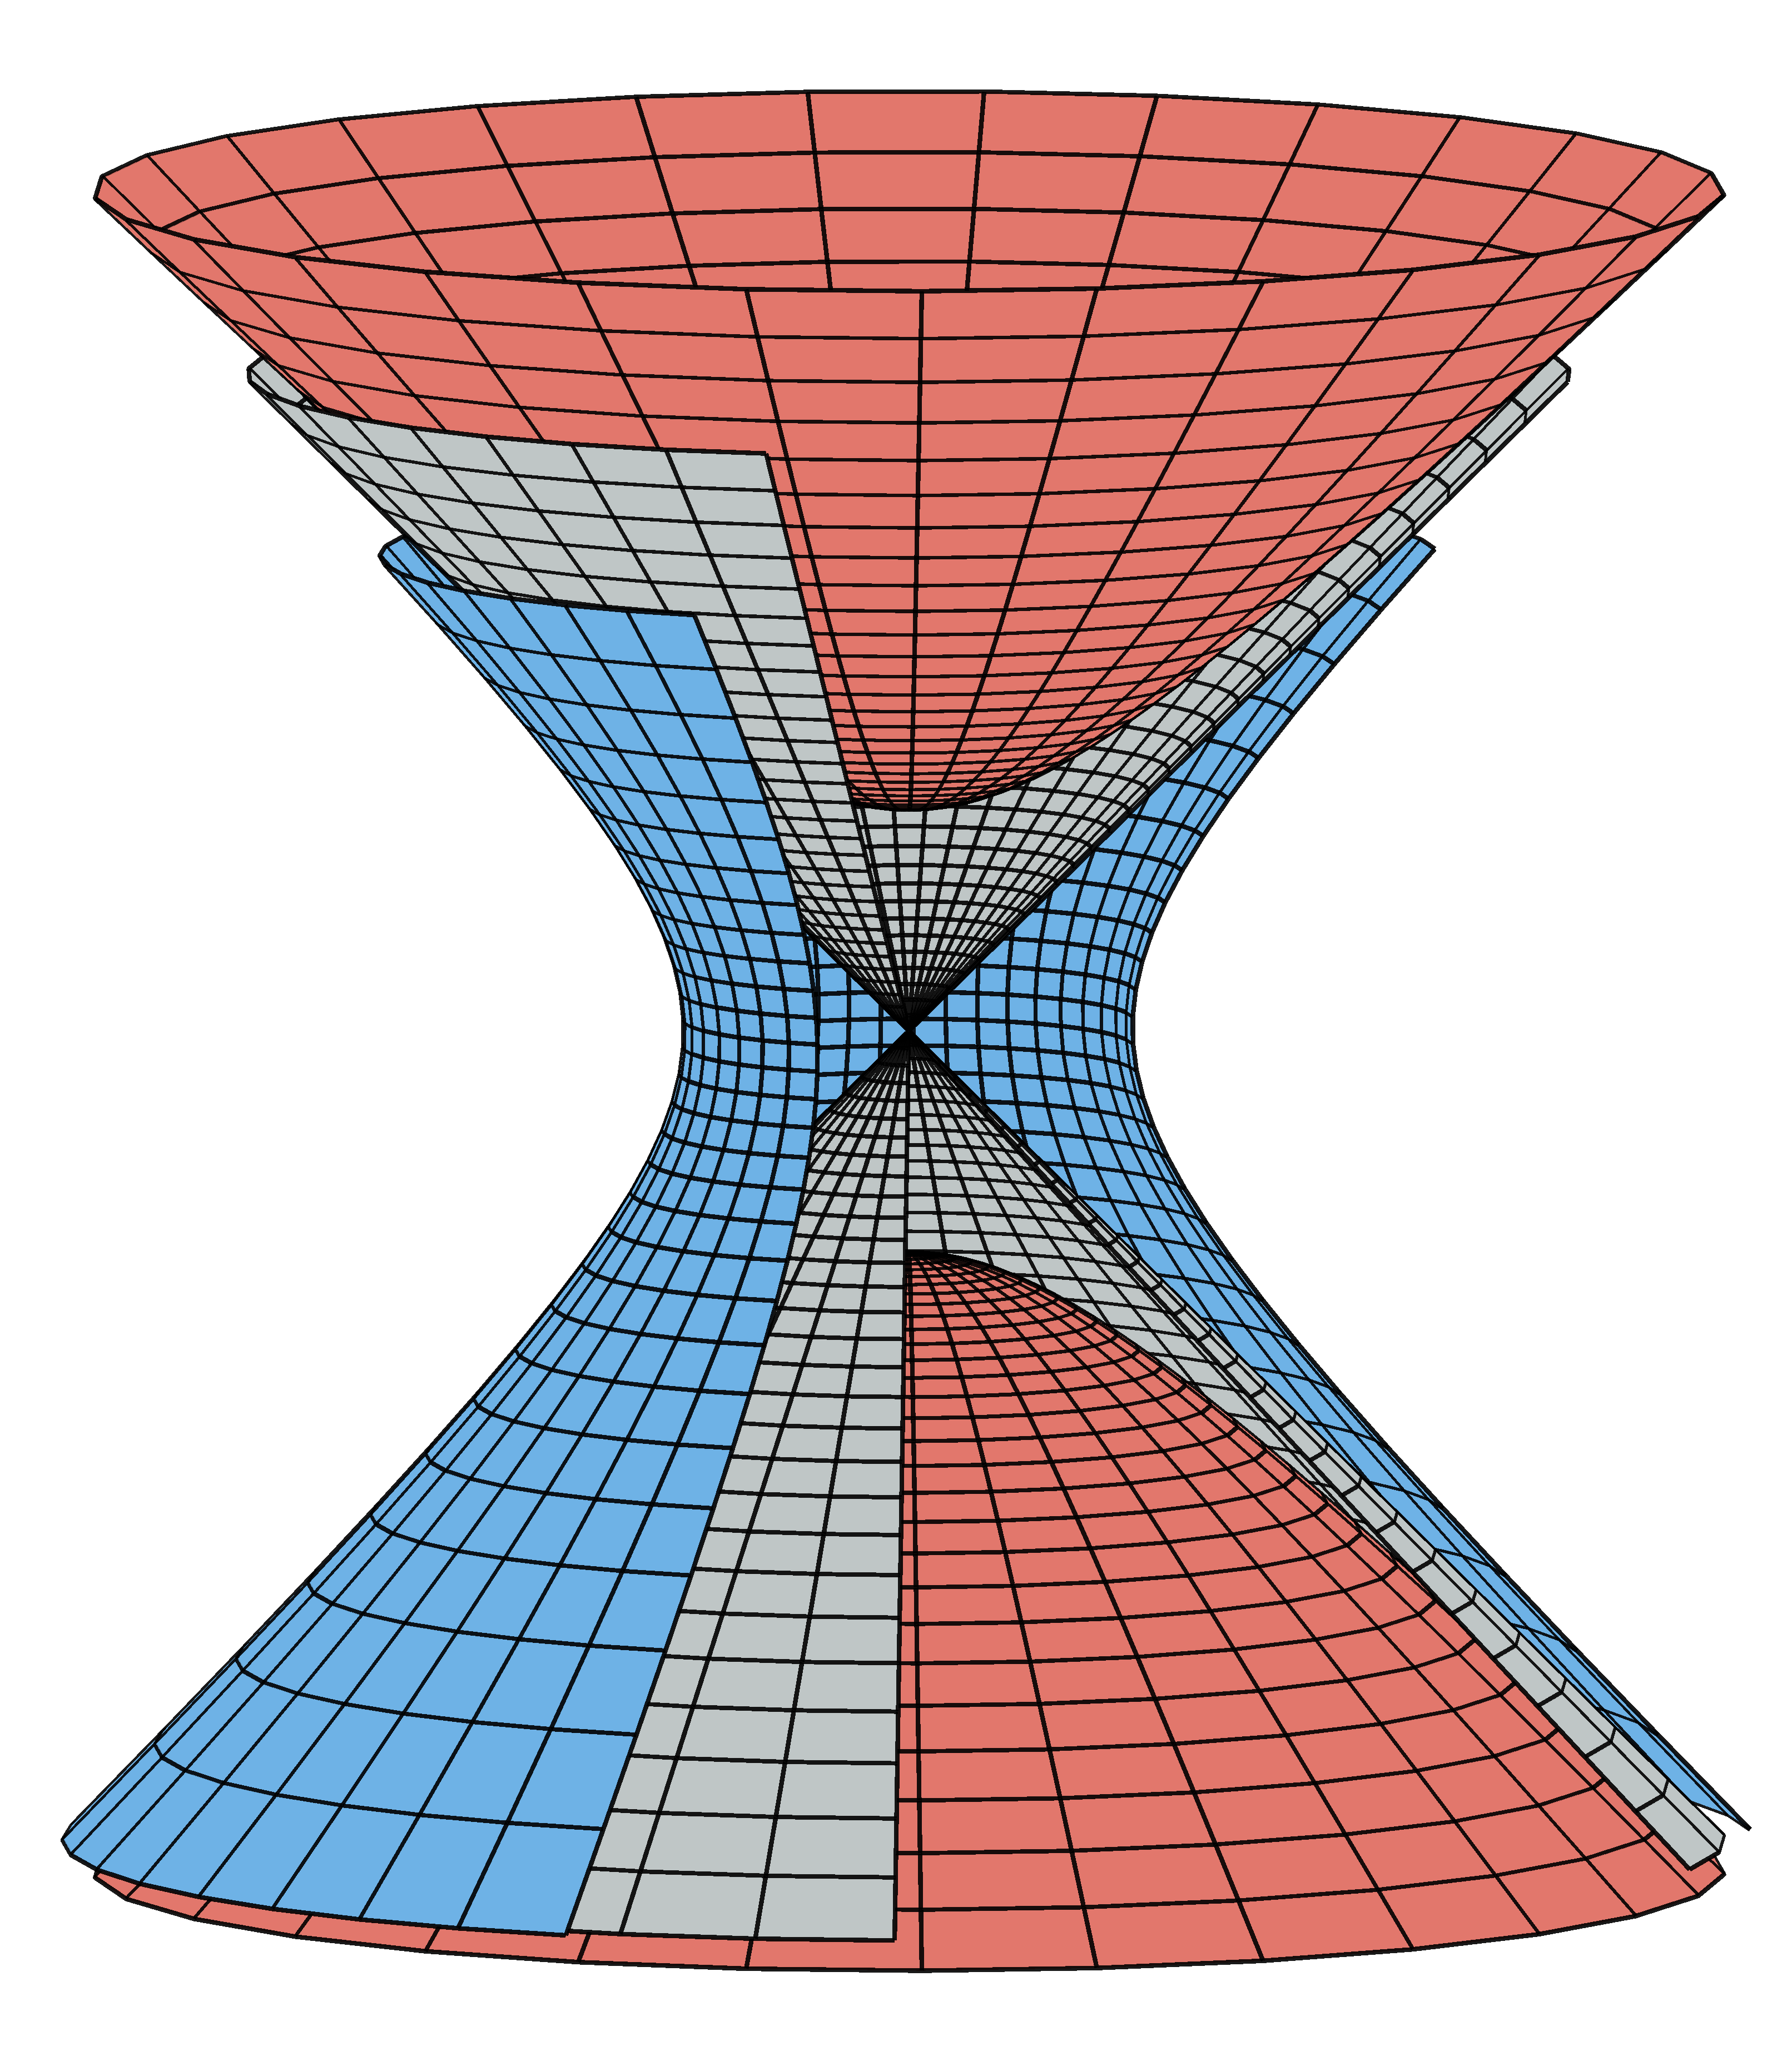
\includegraphics[]{media/other/lorentz_space.png}
    \caption{The disconnected `unit sphere' in the Lorentzian 3-space. The blue surface is the one-sheet hyperboloid, containing all the spacelike unit vectors; the gray sheet is the light cone, that contains all the lightlike `null' vectors with zero norm. Finally, the red surface is the two-sheet hyperboloid, which is the space of all timelike unit vectors.}
    \label{fig:hyperboloids}
\end{figure}

Given the regime of the mechanical systems, the eigenvectors of the state transition matrix determine the particular shape of the trajectories in the phase plane. We distinguish three types of shapes:
\begin{itemize}
    \item[\circled{1}] Saddle point: two directions
    \item[\circled{2}] Stable line: two direction (?)
    \item[\circled{3}] Pure translation: translation direction?
    \item[\circled{4}] Node: two directions
    \item[\circled{6}] A center/spiral, which has elliptic trajectories. These also include the spiral nodes, since the scalar part (contraction) is not part of the vector. We can characterize the shape of the elliptic trajectories by the \emph{eccentricity} and their \emph{tilt} (i.e. the rotation of the major axes of the ellipse with respect to the phase plane axes). 
\end{itemize}

Compute real eigenvectors by substituting the action of multiplying with a vector \emph{in} the split-quaternion and solving appropriately.

\subsubsection{Underdamped systems}

\begin{figure}
    \centering
    \begin{tikzpicture}[scale=1.5]

    \draw[thin,->] (0, -1.5) -- (0, 4) node[anchor=south] {$i$};
    \draw[thin,->] (-4, 0) -- (4, 0) node[anchor=west] {$j$};

    \draw [semithick, smooth, samples=100 ,domain=-2:2] plot({sinh(\x)}, {cosh(\x)});
    
    %\draw[dashed] (1, 0) arc (0:180:1);
    %\draw[dashed] (1, 0) -- (1, 3);

    \draw[thick, name path=pdisk] (-1, 0) node[circle, draw, fill=white, inner sep = 0.3mm] {} -- (1, 0) node[circle, draw, fill=white, inner sep = 0.3mm] {}; 

    \draw[thick, name path=cdisk] (-1, 1) node[circle, draw, fill=white, inner sep = 0.3mm] {} -- (1, 1) node[circle, draw, fill=white, inner sep = 0.3mm] {}; 
    
    \node[] (p) at (0, -1) {-};
    
    \node[circle, fill=black, draw, inner sep = 0.3mm] (x) at ({sinh(-1.3)}, {cosh(-1.3)}) {};
    \node[] (x) (o) at (0, 0) {};
    
    \draw[thin, name path = pdisk_proj] (x) -- (p.center);
    \draw[thin, name path = cdisk_proj] (x) -- (o.center);
    
    \path [name intersections={of=pdisk_proj and pdisk,by=e}];
    \path [name intersections={of=cdisk_proj and cdisk,by=f}];
    
    \node[circle, fill=black, draw, inner sep = 0.3mm]  at (e) {};
    \node[circle, fill=black, draw, inner sep = 0.3mm]  at (f) {};
    %\node[circle, fill=black, draw, inner sep = 0.3mm]  at (f) {};
    
    \node[anchor=west] at (p) {\footnotesize{$-1$}};
    \node[anchor=north west, outer sep=1mm] at (1, 0) {\footnotesize{$1$}};
    \node[anchor=north east, outer sep=1mm] at (-1, 0) {\footnotesize{$-1$}};
    
    \path[->] (e) |- node (rpc) {} (0, 1.5);
    \path[->] (f) |- node (rk) {} (0, 2);
    
    \draw[dotted, very thin] (e) ++(0, 0.1) -- (rpc);
    \draw[dotted, very thin] (f) ++(0, 0.1) -- (rk);
    
    \draw[->|] (0, 1.5) -- (rpc.center) node[pos=0.5, anchor=south] {\footnotesize $r_\text{pc}$};
    \draw[->|] (0, 2) -- (rk.center) node[pos=0.5, anchor=south] {\footnotesize $r_\text{k}$};
    
    \node[anchor=north west] at (0.5, 1) {\scriptsize \textsc{Cayley-Klein}};
    \node[anchor=south west] at (0.5, 0) {\scriptsize \textsc{Poincaré}};
    
    \draw[thick] (0, -3.3) circle (1);
    
    \draw[dotted, very thin] (-1, 1) -- (-1, -3.3); 
    \draw[dotted, very thin] (1, 1) -- (1, -3.3); 
    \draw[thin, ->] (0, -3.3) ++(0, -1.3) -- ++ (0, 2.6) node[anchor = west] {$k$};
    \draw[thin, ->] (0, -3.3) ++(-1.3, 0) -- ++ (2.6, 0) node[anchor = west] {$i$};
    
    \draw[dotted, very thin] (e) -- ++(0, -3.3) node[circle, fill=black, draw, inner sep = 0.3mm] {}; 
    \draw[dotted, very thin] (f) -- ++(0, -4.3) node[circle, fill=black, draw, inner sep = 0.3mm] {};
    
\end{tikzpicture}

    \caption{Illustration of the projection on the Poincaré disk and the Cayley-Klein disk.}
    \label{fig:hyperboloid_projection}
\end{figure}

\todo{Master figure with multiple trajectories and their respective locations on the poincaré disk, with poincaré disk as map}

\FloatBarrier
\section{Notes}
! orthogonal refers to `regular' orthogonal, Lorentz-orthogonal makes the distinction.

Motivation: $\vec{u}$ seems to be `aligned' with major direction of the elliptic trajectory in the Lorentz-orthogonal subspace, generated by the action of its cross-product. Show this formally by making use of the eigenvectors.

The basis vectors $ \qty{\vec{e}_2, \vec{e}_3}$, where $\vec{e}_2$ is the orthogonal projection of the vector $\vec{e}_1 = \uvec{u}$ on its Lorentz-orthogonal subspace, and $\vec{e}_3 \triangleq \lorcrossp{\vec{e}_1}{\vec{e}_2}$, form the real and imaginary parts of two of the eigenvectors of the matrix $\mat{U}_{\lorcrossp{}{}}$. 

Because the basis vectors $\vec{e}_2$ and $\vec{e}_3$ are also orthogonal in the Euclidean sense, the 

\begin{proof}
    Let $\uvec{u} = u_1\uvec{i} + u_2\uvec{j} + u_3\uvec{k}$. A normal vector to the Lorentz-orthogonal subspace is $
    \uvec{n} = u_1\uvec{i} - u_2\uvec{j} - u_3\uvec{k}$. Then, the basis vectors are
    \begin{equation}
        \begin{split}
            \vec{e}_2 &= 
            \uvec{u} - \frac{ \inner{\uvec{u}}{\uvec{n}} }{ \inner{\uvec{n}}{\uvec{n}} } \uvec{n} \\
            \vec{e}_3 &= \lorcrossp{\uvec{u}}{\vec{e}_2} = -\frac{ \inner{\uvec{u}}{\uvec{n}} }{ \inner{\uvec{n}}{\uvec{n}} } \qty(\lorcrossp{\uvec{u}}{\uvec{n}}),
        \end{split}
    \end{equation}
    because the Lorentz-cross product distributes over addition and $\lorcrossp{\uvec{u}}{\uvec{u}} = \vec{0}$. The proposition above claims that $\vec{e}_2 + \ii\vec{e}_3$ is an eigenvector of the matrix $\mat{U}_{\lorcrossp{}{}}$. Hence, it must be the case that $\mat{U}_{\lorcrossp{}{}}(\vec{e}_2 + \ii\vec{e}_3) = \lambda(\vec{e}_2 + \ii\vec{e}_3)$, where $\lambda$ is then an eigenvalue of the matrix. This can be verified by replacing the action of $\mat{U}_{\lorcrossp{}{}}$ with the cross product. Plugging in the definition and exploiting the linearity of the Lorentz cross-product, we obtain:
    \begin{equation*}
        \begin{split}
            \lorcrossp{\uvec{u}}{\qty(\vec{e}_2 + \ii\vec{e}_3)} 
            &= \lorcrossp{\uvec{u}}{\vec{e}_2} +
        \ii\qty(\lorcrossp{\uvec{u}}{\vec{e}_3}) \\
            &= \vec{e}_3 + \qty(\lorcrossp{\uvec{u}}{\vec{e}_3})\ii \\ 
            &=\vec{e}_3 +  \qty(\lorcrossp{\uvec{u}}{\qty(\lorcrossp{\uvec{u}}{\vec{e}_2})})\ii \\
            &=\vec{e}_3 -  \frac{ \inner{\uvec{u}}{\uvec{n}} }{ \inner{\uvec{n}}{\uvec{n}} }\qty(\lorcrossp{\uvec{u}}{\qty(\lorcrossp{\uvec{u}}{\uvec{n}})})\ii.  \\
        \end{split}
    \end{equation*}
The triple cross-product expansion, or `Lagrange formula', relates the regular cross product to the corresponding dot product:
    $$ \vec{a}\times\qty(\vec{b}\times\vec{c}) = \vec{b}\:\inner{\vec{c}}{\vec{a}} - \vec{c}\:\inner{\vec{a}}{\vec{b}}. $$
This well-known identity generalizes (easily verified) to the Lorentzian counterpart of the cross- and inner products:
    $$ 
        \lorcrossp{\vec{a}}{\qty(\lorcrossp{\vec{b}}{\vec{c}})} 
       = \vec{b}\:\lorinner{\vec{c}}{\vec{a}} - \vec{c}\:\lorinner{\vec{a}}{\vec{b}}. 
    $$
Using the Lagrange formula, the above expression becomes
    \begin{equation*}
        \begin{split}
            & \vec{e}_3 - \frac{ \inner{\uvec{u}}{\uvec{n}} }{ \inner{\uvec{n}}{\uvec{n}} }\qty(\uvec{u}\,\lorinner{\uvec{u}}{\uvec{n}} - \uvec{n}\lorinner{\uvec{u}}{\uvec{u}})\ii \\
            & =\, \vec{e}_3 - \qty(\uvec{u}\,\frac{ \lorinner{\uvec{u}}{\uvec{n}} \, \inner{\uvec{u}}{\uvec{n}} }{ \inner{\uvec{n}}{\uvec{n}} } - \uvec{n}\frac{ \inner{\uvec{u}}{\uvec{n}} }{ \inner{\uvec{n}}{\uvec{n}} })\ii \\
            & =\, \vec{e}_3 - \qty(\uvec{u} - \uvec{n}\frac{ \inner{\uvec{u}}{\uvec{n}} }{ \inner{\uvec{n}}{\uvec{n}} })\ii \\
            & =\, \vec{e}_3 - \vec{e}_2\ii. 
        \end{split}
    \end{equation*}
    The latter is the scalar multiple of the vector $\vec{e}_2 + \vec{e}_3$ by $-\ii$ - hence, this is indeed an eigenvector of the corresponding matrix.
\end{proof}
Because $\vec{e}_2$ and $\vec{e}_3$ are also orthogonal in the normal sense, they are aligned with the major axes of the elliptic trajectories generated by the cross product. Hence, they can be used to find a basis of the invariant subspace which makes the trajectories identical to those in the phase plane.

\subsection{Relation with complex Hamiltonians}
\label{ssec:complex_ham}
